% \documentclass[onlytextwidth]{beamer}
\usepackage[utf8]{inputenc}
\usepackage{microtype}
\usepackage{amsmath}
\usepackage{amssymb}
\usepackage[nomessages]{fp} %\FPeval{\var-name}{2*sin(pi/6)}
\usepackage{siunitx} %units in math. eg 20\milli\meter
\usepackage{yhmath} % for arcs, overparenth command
\usepackage{tikz} %graphics
\usetikzlibrary{quotes, angles, arrows, arrows.meta}
%\usepackage{graphicx} already loaded by beamer class
%consider setting \graphicspath{{images/}}
%\parskip ?? to avoid paragraph indent
\usepackage{multicol} %may not need this package, just columns environment
\usepackage{venndiagram}

\subtitle[BECA]{Bronx Early College Academy}
\author[Huson]{Christopher J. Huson PhD}

\setbeamertemplate{headline}{\vskip2mm 
  BECA / \insertshortauthor \, / \inserttitle
  \hfill 
  \insertsection
  }

\title{Geometry Unit 3: Transversals}
\date{11 October - 21 October 2022}

\begin{document}
\frame{\titlepage}
\section[Outline]{}
\frame{\tableofcontents}

\section{3.1 Identify transversal angles \hfill 11 October}
\begin{frame}{Learning Target: I can name parallel lines transversal angles}
  {HSG.CO.C.9 Prove theorems about lines and angles  \hfill \alert{3.1 Tuesday 11 October}}
  \begin{block}{Do Now: Identify the true statements}
    \begin{multicols}{2}
    \begin{enumerate}
      \item $\angle 1 \cong \angle 2$
      \item $\angle 2 \cong \angle 4$
      \item m$\angle 1 + \text{m}\angle 4=180^\circ$
      \item m$\angle 2 + \text{m}\angle 3=90^\circ$
  \end{enumerate}
  \begin{center}
  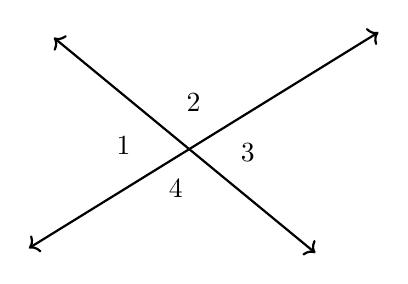
\begin{tikzpicture}[scale=0.5, rotate=15]
    \draw[<->, thick] (0,-1.5)--(10,1.5);
    \draw[<->, thick] (2,3.5)--(7,-3.5);
    \node at (3,.4){1};
    \node at (6,-.6){3};
    \node at (5,1){2};
    \node at (4,-1){4};
  \end{tikzpicture}
  \end{center}
\end{multicols}
\end{block}
    Review: Angle postulates and theorems you have learned. 
    \begin{enumerate}
      \item $\perp$ lines and complementary $\angle$s make $90^\circ$
      \item linear pairs add to $180^\circ$
      \item vertical $\angle$s are $\cong$
      \item definition of an angle bisector
      %\item isosceles base angle theorem
    \end{enumerate}
\end{frame}

\begin{frame}{New terminology for parallel lines}
  {Parallel lines are in the same plane and never intersect}
    \begin{multicols}{2}
      \begin{enumerate}
        \item \emph{parallel lines}, symbol: $\parallel$ tick marks
        \item \emph{transversal line}
        \item \emph{interior, exterior} $\angle$s
        \item \emph{same-side, alternate} $\angle$s
        \item Horizontal and vertical
      \end{enumerate}
        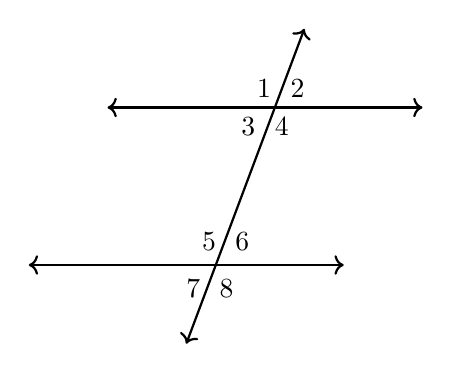
\begin{tikzpicture}[scale=1]
        \draw[<->, thick] (3,2)--(7,2);
        \draw[<->, thick] (2,0)--(6,0);
        \draw[<->, thick] (4,-1)--(5.5,3);
        \node at (4.5,0.3) [left]{$5$};
        \node at (4.5,0.3) [right]{$6$};
        \node at (4.3,-0.3) [left]{$7$};
        \node at (4.3,-0.3) [right]{$8$};
        \node at (5.2,2) [above left]{$1$};
        \node at (5.2,2) [above right]{$2$};
        \node at (5,2) [below left]{$3$};
        \node at (5,2) [below right]{$4$};
      \end{tikzpicture}
    \end{multicols}
  \end{frame}

\begin{frame}{New theorems for parallel lines}
  \begin{multicols}{2}
    \begin{enumerate}
      \item \emph{corresponding} $\angle$s of $\parallel$ lines are $\cong$\\
        $\angle 2 \cong \angle 6$
      \item \emph{same-side interior} $\angle$s are supplementary\\
      m$\angle 3 + \text{m}\angle 5 =  180$
      \item \emph{alternate exterior} $\angle$s are $\cong$\\
      $\angle 2 \cong \angle 7$
    \end{enumerate}
      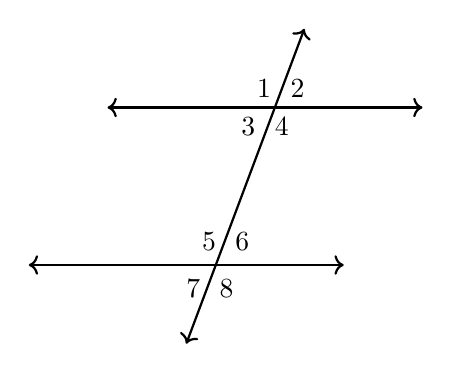
\begin{tikzpicture}[scale=1]
      \draw[<->, thick] (3,2)--(7,2);
      \draw[<->, thick] (2,0)--(6,0);
      \draw[<->, thick] (4,-1)--(5.5,3);
      \node at (4.5,0.3) [left]{$5$};
      \node at (4.5,0.3) [right]{$6$};
      \node at (4.3,-0.3) [left]{$7$};
      \node at (4.3,-0.3) [right]{$8$};
      \node at (5.2,2) [above left]{$1$};
      \node at (5.2,2) [above right]{$2$};
      \node at (5,2) [below left]{$3$};
      \node at (5,2) [below right]{$4$};
    \end{tikzpicture}
  \end{multicols}
  Hint: There are only two angle measures, the acute angles and the obtuse angles\\ (and they add to $180^\circ$)
\end{frame}

\begin{frame}{New theorems for parallel lines}
  Given two parallel lines and a transversal, as shown, with m$\angle 6 =  70^\circ$. Write down the value of each angle measure.
  \begin{multicols}{3}
    \begin{enumerate}[itemsep=0.5cm]
      \item m$\angle 1 = $
      \item m$\angle 2 = $
      \item m$\angle 3 = $
      \item m$\angle 4 = $
      \item m$\angle 5 = $
      \item m$\angle 6 = $
      \item m$\angle 7 = $
      \item m$\angle 8 = $
    \end{enumerate}
      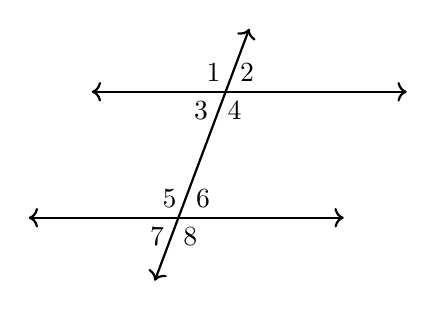
\begin{tikzpicture}[scale=0.8]
      \draw[<->, thick] (3,2)--(8,2);
      \draw[<->, thick] (2,0)--(7,0);
      \draw[<->, thick] (4,-1)--(5.5,3);
      \node at (4.5,0.3) [left]{$5$};
      \node at (4.5,0.3) [right]{$6$};
      \node at (4.3,-0.3) [left]{$7$};
      \node at (4.3,-0.3) [right]{$8$};
      \node at (5.2,2) [above left]{$1$};
      \node at (5.2,2) [above right]{$2$};
      \node at (5,2) [below left]{$3$};
      \node at (5,2) [below right]{$4$};
    \end{tikzpicture}
  \end{multicols}


\end{frame}


\section{3.2 Transversals problems \hfill 12 October}
\begin{frame}{Learning Target: I can calculate transversal angles}
  {HSG.CO.C.9 Prove theorems about lines and angles  \hfill \alert{3.2 Wednesday 12 October}}
  \begin{block}{Do Now: Identify each angle}
    \begin{multicols}{2}
    \begin{enumerate}
      \item Opposite $\angle 4$
      \item Corresponding to $\angle 3$
      \item Alternate exterior to $\angle 8$
      \item Same side interior to $\angle 5$
      \item Alternate interior to $\angle 4$
  \end{enumerate}
  \begin{center}
    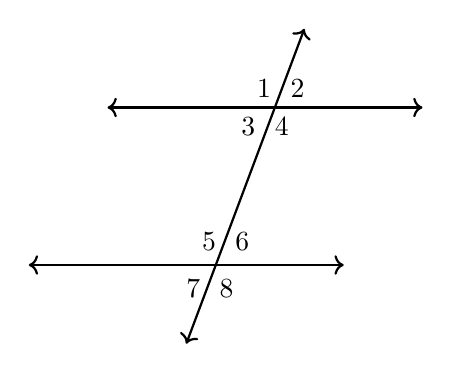
\begin{tikzpicture}[scale=1]
      \draw[<->, thick] (3,2)--(7,2);
      \draw[<->, thick] (2,0)--(6,0);
      \draw[<->, thick] (4,-1)--(5.5,3);
      \node at (4.5,0.3) [left]{$5$};
      \node at (4.5,0.3) [right]{$6$};
      \node at (4.3,-0.3) [left]{$7$};
      \node at (4.3,-0.3) [right]{$8$};
      \node at (5.2,2) [above left]{$1$};
      \node at (5.2,2) [above right]{$2$};
      \node at (5,2) [below left]{$3$};
      \node at (5,2) [below right]{$4$};
    \end{tikzpicture}
  \end{center}
\end{multicols}
\end{block}
Lesson: Triangle sum theorem
\end{frame}

\section{3.3 Transversal situations \hfill 13 October}
\begin{frame}{Learning Target: I can calculate transversal angles}
  {HSG.CO.C.9 Prove theorems about lines and angles  \hfill \alert{3.3 Thursday 13 October}}
  Given two parallel lines and a transversal, with m$\angle 4 = 3x$ and m$\angle 5 = x + 70$. \\ Write an equation, then solve for $x$.
  \begin{flushright}
    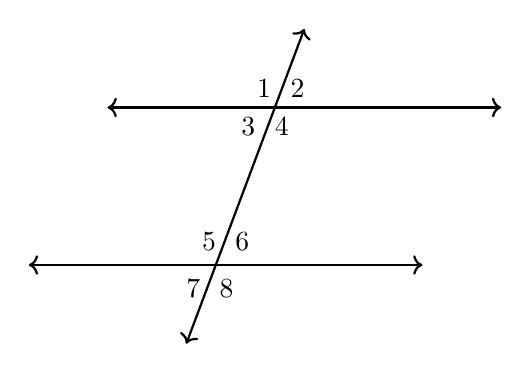
\begin{tikzpicture}[scale=1]
      \draw[<->, thick] (3,2)--(8,2);
      \draw[<->, thick] (2,0)--(7,0);
      \draw[<->, thick] (4,-1)--(5.5,3);
      \node at (4.5,0.3) [left]{$5$};
      \node at (4.5,0.3) [right]{$6$};
      \node at (4.3,-0.3) [left]{$7$};
      \node at (4.3,-0.3) [right]{$8$};
      \node at (5.2,2) [above left]{$1$};
      \node at (5.2,2) [above right]{$2$};
      \node at (5,2) [below left]{$3$};
      \node at (5,2) [below right]{$4$};
    \end{tikzpicture}
  \end{flushright}
\end{frame}

\section{3.4 Parallelograms \hfill 14 October}
\begin{frame}{Learning Target: I can define a parallelogram}
  {HSG.CO.C.9 Prove theorems about lines and angles  \hfill \alert{3.4 Friday 14 October}}
  Two parallel lines intersect a transversal. Given corresponding angles  m$\angle 1 = 4.4x - 63$ and m$\angle 2 = 2.8x+9$, find the measure of $\angle 1$. 
  \begin{flushright}
    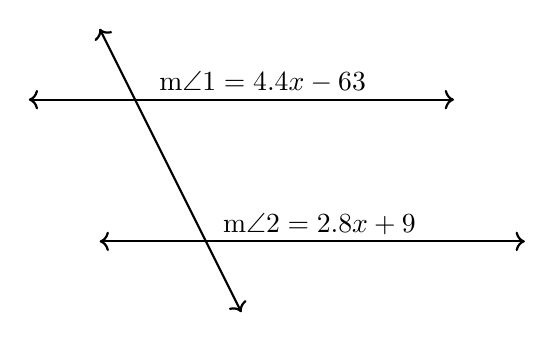
\begin{tikzpicture}[scale=0.9]
      \draw[<->, thick] (3,0)--(9,0);
      \draw[<->, thick] (2,2)--(8,2);
      \draw[<->, thick] (5,-1)--(3,3);
      %\draw[<->, thick] (11,-1)--(9,3);
      %\node at (4, 1.7){$1$};
      \node at (5.3, 2.25){m$\angle 1 = 4.4x - 63$};
      \node at (6.1, 0.25){m$\angle 2 = 2.8x+9$};
      %\node at (10, 0.25){$3$};
    \end{tikzpicture}
    \end{flushright}
\end{frame}

\section{3.5 Triangle sum proof \hfill 17 October}
\begin{frame}{Learning Target: I can calculate triangle angles}
  {HSG.CO.C.9 Prove theorems about lines and angles  \hfill \alert{3.5 Monday 17 October}}

\end{frame}

\section{3.6 External angles \hfill 18 October}
\begin{frame}{Learning Target: I can calculate external triangle angles}
  {HSG.CO.C.9 Prove theorems about lines and angles  \hfill \alert{3.6 Tuesday 18 October}}
  Do Now: 
  \begin{multicols}{2}
    \begin{enumerate}
      \item Given two parallel lines, two transversals
      \item Find $x$, $y$
      \item What relationship are you using? (e.g. vertical angles, same-side exterior angles, alternate interior angles, etc.)
    \end{enumerate}
      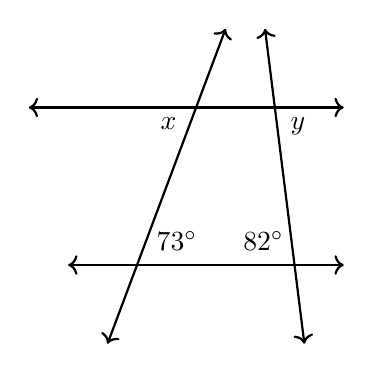
\begin{tikzpicture}[scale=1]
      \draw[<->, thick] (3,2)--(7,2);
      \draw[<->, thick] (3.5,0)--(7,0);
      \draw[<->, thick] (4,-1)--(5.5,3);
      \draw[<->, thick] (6.5,-1)--(6,3);
      \node at (4.5,0.3) [right]{$73^\circ$};
      \node at (5.6,0.3) [right]{$82^\circ$};
      \node at (5,2) [below left]{$x$};
      \node at (6.2,2) [below right]{$y$};
    \end{tikzpicture}
  \end{multicols}
  Lesson: Sum of a triangle's interior angles is $180^\circ$ \\[0.25cm]
  Homework: Deltamath 3.6 (Marking Period ends tomorrow)
\end{frame}


\begin{frame}
    Given parallel lines $\overleftrightarrow{AB} \parallel \overleftrightarrow{CDE}$ with $\overline{AC} \cong \overline{CD}$. If m$\angle BAD=80$ find m$\angle ACD$.
  \begin{flushright}
  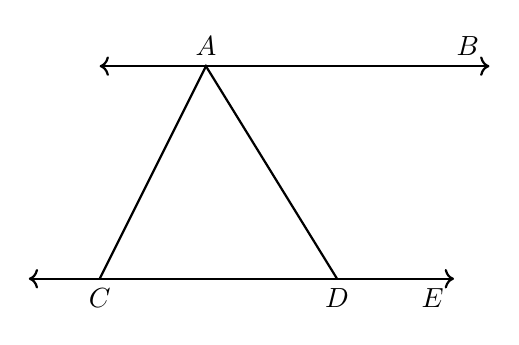
\begin{tikzpicture}[scale=0.9]
    \draw[<->, thick] (1,3)--(6.5,3) node[above left]{$B$};
    \draw[<->, thick] (0,0)--
      (5,0)--
      (6,0) node[below left]{$E$};
    \draw[-, thick] (1,0) node[below]{$C$}--
      (2.5,3) node[above]{$A$}--
      (4.35,0) node[below]{$D$};
  \end{tikzpicture}
  \end{flushright} \vspace{1cm}
  \end{frame}

\section{3.7 Parallelogram situations \hfill 19 October}
\begin{frame}{Learning Target: I can calculate angles in parallelograms}
  {HSG.CO.C.9 Prove theorems about lines and angles  \hfill \alert{3.7 Wednesday 19 October}}
  Do Now: 
  \begin{multicols}{2}
    \begin{enumerate}
      \item Given a triangle, shown
      \item Find $x$, $y$
      \item What relationships are you using? (e.g. vertical angles, same-side exterior angles, alternate interior angles, etc.)
    \end{enumerate}
    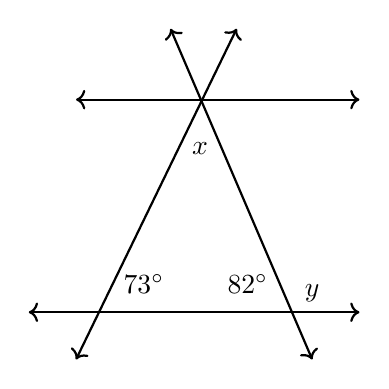
\begin{tikzpicture}[scale=1.2]
      \draw[<->, thick] (4,2.25)--(7,2.25);
      \draw[<->, thick] (3.5,0)--(7,0);
      \draw[<->, thick] (4,-0.5)--(5.7,3);
      \draw[<->, thick] (6.5,-0.5)--(5,3);
      \node at (4.4,0.3) [right]{$73^\circ$};
      \node at (5.5,0.3) [right]{$82^\circ$};
      \node at (5.5,1.9) [below left]{$x$};
      \node at (6.5,0.2) {$y$};
    \end{tikzpicture}
  \end{multicols}
  Lesson: Triangle's exterior angles
\end{frame}

\section{3.8 Transversals review \hfill 20 October}
\begin{frame}{Learning Target: I can review with my classmates}
  {HSG.CO.C.9 Prove theorems about lines and angles \hfill \alert{3.8 Thursday 20 October}}
  Two parallel lines intersect a second set of parallel lines. Given m$\angle 2 = 2.8x+9$ and m$\angle 4 = 4.4x - 63$, find the measure of $\angle 1$. 
  \begin{flushright}
    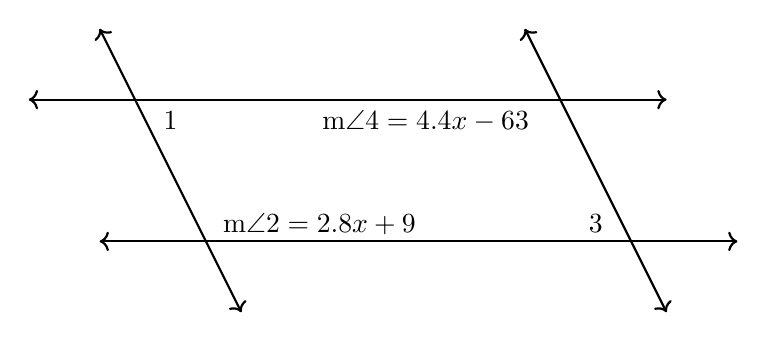
\begin{tikzpicture}[scale=0.9]
      \draw[<->, thick] (3,0)--(12,0);
      \draw[<->, thick] (2,2)--(11,2);
      \draw[<->, thick] (5,-1)--(3,3);
      \draw[<->, thick] (11,-1)--(9,3);
      \node at (4, 1.7){$1$};
      \node at (6.1, 0.25){m$\angle 2 = 2.8x+9$};
      \node at (10, 0.25){$3$};
      \node at (7.6, 1.7){m$\angle 4 = 4.4x - 63$};
    \end{tikzpicture}
    \end{flushright}
\end{frame}

\section{3.9 Transversals test \hfill 21 October}
\begin{frame}{Learning Target: I can review with my classmates}
  {HSG.CO.C.9 Prove theorems about lines and angles \hfill \alert{3.9 Friday 21 October}}

\end{frame}


\end{document}